\section{NHIỆT DUNG RIÊNG}
\subsection{LÝ THUYẾT TRỌNG TÂM}
\subsubsection{Nhiệt dung riêng}
\begin{boxdn}
	Nhiệt dung riêng của một chất là nhiệt lượng cần cung cấp để nhiệt độ của $\SI{1}{\kilogram}$ chất đó tăng thêm $\SI{1}{\kelvin}$.
\end{boxdn}
Đơn vị đo của nhiệt dung riêng trong hệ SI là $\si{\joule/\left(\kilogram\cdot\kelvin\right)}$, nhiệt dung riêng kí hiệu là $c$.
\subsubsection{Nhiệt lượng trao đổi để khối chất thay đổi nhiệt độ}
\begin{boxdn}
	Nhiệt lượng trao đổi (toả ra hay nhận vào) để khối chất thay đổi nhiệt độ từ $T_1$ đến nhiệt độ $T_2$:
	$$Q=mc\Delta T$$
\end{boxdn}
với:
\begin{itemize}
	\item $Q$: nhiệt lượng trao đổi, đơn vị trong hệ SI là $\si{\joule}$;
	\item $m$: khối lượng, đơn vị trong hệ SI là $\si{\kilogram}$;
	\item $c$: nhiệt dung riêng của chất tạo nên vật, đơn vị trong hệ SI là $\si{\joule/\left(\kilogram\cdot\kelvin\right)}$;
	\item $\Delta T=T_2-T_1$: độ biến thiên nhiệt độ, đơn vị trong hệ SI là $\si{\kelvin}$.
\end{itemize}
\subsubsection{Trạng thái cân bằng nhiệt của hệ nhiệt động}
\begin{boxdn}
	Hệ nhiệt động đạt trạng thái cân bằng nhiệt khi tổng nhiệt lượng trao đổi trong hệ bằng 0:
	$$\sum Q=Q_1+Q_2+\dots+Q_n=0.$$
\end{boxdn}
\subsection{VÍ DỤ MINH HOẠ}
\begin{dang}{Xác định nhiệt lượng trao đổi để khối chất thay đổi nhiệt độ}
	\end{dang}
	\begin{vd}
		Hãy giải thích tại sao ban ngày có gió mát thổi từ biển vào đất liền? Biết rằng nhiệt dung riêng của đất và nước vào khoảng $\SI{800}{\joule/\left(\kilogram\cdot\kelvin\right)}$ và $\SI{4200}{\joule/\left(\kilogram\cdot\kelvin\right)}$.
	\loigiai{Vào ban ngày, vì nhiệt dung riêng của nước cao hơn nhiệt dung riêng của đất nên với cùng nhiệt lượng nhận từ Mặt Trời thì nước biển có độ tăng nhiệt độ thấp hơn đất liền. Do hiện tượng đối lưu, luồng không khí từ biển sẽ thổi vào đất liền. Lúc này có sự trao đổi nhiệt lượng giữa không khí trong đất liền và không khí từ biển thổi vào làm giảm nhiệt độ không khí ở đất liền. Do đó, chúng ta sẽ cảm thấy mát hơn}

	\end{vd}
	
	
\begin{vd}
Một thùng đựng $\SI{20}{\ell}$ nước ở nhiệt độ $\SI{20}{\celsius}$. Cho khối lượng riêng của nước là $\SI{1000}{\kilogram\cdot\meter^{-3}}$, nhiệt dung riêng của nước $c=\SI{4200}{\joule/\left(\kilogram\cdot\kelvin\right)}$.
			\begin{enumerate}[label=\alph*)]
				\item Tính nhiệt lượng cần truyền cho nước trong thùng để nhiệt độ của nó tăng lên tới $\SI{70}{\celsius}$.
				\item Tính thời gian truyền nhiệt lượng cần thiết nếu dùng một thiết bị điện có công suất $\SI{2.5}{\kilo\watt}$ để đun lượng nước trên. Biết chỉ có $\SI{80}{\percent}$ điện năng tiêu thụ được dùng để làm nóng nước.
			\end{enumerate}
	\loigiai{
				\begin{enumerate}[label=\alph*)]
					\item Khối lượng của $\SI{20}{\ell}$ nước:
					$$m=\rho V=\left(\SI{1000}{\kilogram\cdot\meter^{-3}}\right)\cdot\left(\SI{20E-3}{\meter^{3}}\right)=\SI{20}{\kilogram}.$$
					Nhiệt lượng cần truyền cho nước trong thùng để nhiệt độ của nó tăng lên tới $\SI{70}{\celsius}$:
					$$Q=mc\Delta t=\left(\SI{20}{\kilogram}\right)\cdot\left[\SI{4200}{\joule/\left(\kilogram\cdot\kelvin\right)}\right]\cdot\left(\SI{50}{\kelvin}\right)=\SI{42E5}{\joule}.$$
					\item Năng lượng thiết bị điện tiêu thụ để truyền được nhiệt lượng cần thiết đun nóng nước đến $\SI{70}{\celsius}$:
					$$W=\dfrac{Q}{H}=\SI{52.5E5}{\joule}.$$
					Thời gian đun nước:
					$$t=\dfrac{W}{\calP}=\dfrac{\SI{52.5E5}{\joule}}{\SI{2.5E3}{\watt}}=\SI{2100}{\second}=\SI{35}{\minute}.$$
				\end{enumerate}}
		
\end{vd}
\begin{dang}{Vận dụng phương trình cân bằng nhiệt}
	\end{dang}
\begin{vd}
		Một bác thợ rèn nhúng một con dao rựa bằng thép có khối lượng $\SI{1.1}{\kilogram}$ ở nhiệt độ $\SI{850}{\celsius}$ vào trong bể nước lạnh để làm tăng độ cứng của lưỡi dao. Nước trong bể có thể tích $\SI{200}{\ell}$ và có nhiệt độ bằng nhiệt độ ngoài trời là $\SI{27}{\celsius}$. Xác định nhiệt độ của nước khi có sự cân bằng nhiệt. Bỏ qua sự truyền nhiệt cho thành bể, môi trường bên ngoài và bỏ qua quá trình nước hoá hơi khi vừa tiếp xúc với rựa. Biết nhiệt dung riêng của thép là $\SI{460}{\joule/\left(\kilogram\cdot\kelvin\right)}$; của nước là $\SI{4180}{\joule/\left(\kilogram\cdot\kelvin\right)}$.
\loigiai{
			Gọi $t_\text{cb}$ là nhiệt độ của nước khi có sự cân bằng nhiệt.\\
			Hệ đạt trạng thái cân bằng nhiệt khi tổng nhiệt lượng trao đổi trong hệ bằng 0:
			\begin{eqnarray*}
				&&	Q_\text{rựa}+Q_\text{nước}=0\\
				&\Leftrightarrow&	m_\text{t}c_\text{t}\left(t_\text{cb}-t_\text{t}\right)+m_\text{n}c_\text{n}\left(t_\text{cb}-t_\text{n}\right)=0\\
				&\Rightarrow& t_\text{cb}=\dfrac{m_\text{n}c_\text{n}t_\text{n}+m_\text{t}c_\text{t}t_\text{t}}{m_\text{n}c_\text{n}+m_\text{t}c_\text{t}}\approx\SI{27.5}{\celsius}.
			\end{eqnarray*}
		}
\end{vd}
	
\begin{vd}
Một bình nhiệt lượng kế bằng nhôm có khối lượng $m_1=\SI{200}{\gram}$ chứa $m_2=\SI{400}{\gram}$ nước ở nhiệt độ $t_1=\SI{20}{\celsius}$. Đổ thêm vào bình một khối lượng nước $m$ ở nhiệt độ $t_2=\SI{5}{\celsius}$. Khi cân bằng nhiệt thì nhiệt độ của nước trong bình là $t=\SI{10}{\celsius}$. Cho biết nhiệt dung riêng của nhôm là $c_1=\SI{880}{\joule/\left(\kilogram\cdot\kelvin\right)}$, của nước là $c_2=\SI{4200}{\joule/\left(\kilogram\cdot\kelvin\right)}$. Bỏ qua sự trao đổi nhiệt với môi trường. Xác định giá trị của $m$.
\loigiai{Khi hệ đạt trạng thái cân bằng nhiệt thì tổng nhiệt lượng trao đổi của hệ bằng 0:
			$$mc_2\left(t-t_2\right)+m_1c_1\left(t-t_1\right)+m_2c_2\left(t-t_1\right)=0$$
			\begin{eqnarray*}
				\Rightarrow m&=&\dfrac{m_1c_1\left(t-t_1\right)+m_2c_2\left(t-t_1\right)}{c_2\left(t_2-t\right)}\\
				&=&\dfrac{\left\{\left(\SI{0.2}{\kilogram}\right)\cdot\left[\SI{880}{\joule/\left(\kilogram\cdot\kelvin\right)}\right]+\left(\SI{0.4}{\kilogram}\right)\cdot\left[\SI{4200}{\joule/\left(\kilogram\cdot\kelvin\right)}\right]\right\}\cdot\left(\SI{10}{\celsius}-\SI{20}{\celsius}\right)}{\left[\SI{4200}{\joule/\left(\kilogram\cdot\kelvin\right)}\right]\cdot\left(\SI{5}{\celsius}-\SI{10}{\celsius}\right)}\\
				&\approx&\SI{0.88}{\kilogram}.
			\end{eqnarray*}
		}
\end{vd}
\subsection{BÀI TẬP TRẮC NGHIỆM}
\setcounter{ex}{0}
\Opensolutionfile{ans}[ans/G12Y24B4TN]
% ===================================================================
\begin{ex}
	Nhiệt lượng vật trao đổi để thay đổi nhiệt độ phụ thuộc vào
	\choice
	{khối lượng, thể tích và độ thay đổi nhiệt độ của vật}
	{ thể tích, nhiệt độ ban đầu và chất cấu tạo nên vật}
	{\True  khối lượng của vật, chất cấu tạo nên vật và độ thay đổi nhiệt độ của vật}
	{nhiệt độ ban đầu, nhiệt độ lúc sau và áp suất của môi trường}
	\loigiai{ }
	\end{ex}
% ===================================================================
\begin{ex}
	Có 4 bình A, B, C, D đều đựng nước ở cùng một nhiệt độ với thể tích tương ứng là: 1 lít, 2 lít, 3 lít, 4 lít. Sau
	khi dùng các đèn cồn giống hệt nhau để đun các bình này khác nhau. Bình có nhiệt độ thấp nhất là
	\begin{center}
		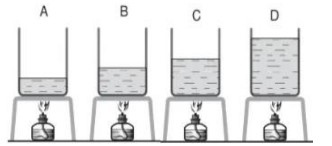
\includegraphics[width=0.4\linewidth]{figs/VN12-Y24-PH-SYL-004P-1}
	\end{center}
	\choice
	{bình A}
	{bình B}
	{bình C}
	{\True bình D}
	\loigiai{}
\end{ex}
% ===================================================================
\begin{ex}
Có 4 bình A, B, C, D đều đựng nước ở cùng một nhiệt độ với thể tích tương ứng là: 1 lít, 2 lít, 3 lít, 4 lít. Sau
khi dùng các đèn cồn giống hệt nhau để đun các bình này khác nhau. Bình có nhiệt độ cao nhất là
\begin{center}
	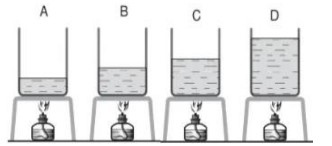
\includegraphics[width=0.4\linewidth]{figs/VN12-Y24-PH-SYL-004P-1}
\end{center}
	\choice
	{\True bình A}
	{bình B}
	{bình C}
	{bình D}
	\loigiai{}
\end{ex}
% ===================================================================
\begin{ex}
	Chọn phát biểu \textbf{sai}.\\
	Nhiệt dung riêng của một chất 
	\choice
	{là nhiệt lượng cần truyền để $\SI{1}{\kilogram}$ chất đó tăng thêm $\SI{1}{\celsius}$}
	{\True phụ thuộc vào khối lượng riêng của chất đó}
	{phụ thuộc vào bản chất của chất đó}
	{có đơn vị là $\si{\joule/\kilogram\cdot\kelvin}$}
	\loigiai{}
\end{ex}
% ===================================================================
\begin{ex}
Nhiệt độ của vật nào tăng lên nhiều nhất khi ta thả rơi bốn vật dưới đây có cùng khối lượng và từ cùng một độ cao xuống đất? Coi như toàn bộ cơ năng của vật chuyển hoá thành nhiệt năng.
	\choice
	{Vật bằng nhôm, có nhiệt dung riêng là $\SI{880}{\joule/\kilogram\cdot\kelvin}$}
	{Vật bằng đồng, có nhiệt dung riêng là $\SI{380}{\joule/\kilogram\cdot\kelvin}$}
	{\True Vật bằng chì, có nhiệt dung riêng là $\SI{120}{\joule/\kilogram\cdot\kelvin}$}
	{Vật bằng gang, có nhiệt dung riêng là $\SI{5500}{\joule/\kilogram\cdot\kelvin}$}
	\loigiai{$$\Delta t=\dfrac{Q}{mc}.$$
		Vì chì có nhiệt dung riêng nhỏ nhất nên có độ tăng nhiệt độ nhiều nhất}
\end{ex}
% ===================================================================
\begin{ex}
	Người ta cọ xát hai vật với nhau, nhiệt dung của hai vật là $\SI{800}{\joule/\kelvin}$. Sau 1 phút người ta thấy nhiệt độ của mỗi vật tăng thêm $\SI{30}{\kelvin}$. Công suất trung bình của việc cọ xát bằng
	\choice
	{$\SI{1080}{\watt}$}
	{$\SI{980}{\watt}$}
	{$\SI{480}{\watt}$}
	{\True $\SI{800}{\watt}$}
	\loigiai{	Công suất trung bình của việc cọ xát là
		$$\calP=\dfrac{2c\Delta T}{t}=\SI{800}{\watt}.$$}
\end{ex}
% ===================================================================
\begin{ex}
	Đầu thép của một búa máy có khối lượng $\SI{12}{\kilogram}$ nóng lên thêm $\SI{20}{\celsius}$ sau 1,5 phút hoạt động. Biết rằng  $\SI{40}{\percent}$ cơ năng của búa máy chuyển thành nhiệt năng của đầu búa. Nhiệt dung riêng của thép là $\SI{460}{\joule/\kilogram\cdot\kelvin}$. Công suất của búa gần nhất với giá trị nào sau đây?
	\choice
	{\True $\SI{3}{\kilo\watt}$}
	{$\SI{4}{\kilo\watt}$}
	{$\SI{5}{\kilo\watt}$}
	{$\SI{6}{\kilo\watt}$}
	\loigiai{		Công suất toả nhiệt trên đầu búa:
		$$\calP_\text{hp}=\dfrac{mc\Delta T}{t}\approx\SI{1226.67}{\watt}.$$
		Công suất của búa:
		$$\calP=\dfrac{\calP_\text{hp}}{0,4}\approx\SI{3.066}{\kilo\watt}.$$}
\end{ex}
% ===================================================================
\begin{ex}
	\immini{Quả cầu kim loại được làm bằng chất có nhiệt dung riêng $c=\SI{460}{\joule/\left(\kilogram\cdot\kelvin\right)}$ được treo bởi sợi day có chiều dài $\ell=\SI{46}{\centi\meter}$. Quả cầu được nâng lên đến B rồi thả rơi. Sau khi chạm tường, nó bật lên đến C $\left(\alpha=\SI{60}{\degree}\right)$. Biết rằng $\SI{60}{\percent}$ độ giảm thế năng của quả cầu biến thành nhiệt làm nóng quả cầu. Lấy $g=\SI{10}{\meter/\second^2}$. Độ tăng nhiệt độ của quả cầu là
\choice
{\True $\SI{3E-3}{\celsius}$}
{$\SI{6E-3}{\celsius}$}
{$\SI{1.5E-3}{\celsius}$}
{Không đủ dữ kiện để xác định}	
}{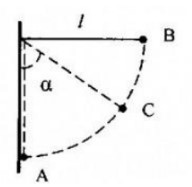
\includegraphics[scale=0.3]{figs/VN12-Y24-PH-SYL-004P-2}
}
	\loigiai{Độ tăng nhiệt độ của quả cầu:
		$$\Delta t=\dfrac{0,6mg\ell\cos\SI{60}{\degree}}{mc}=\dfrac{0,6g\ell\cos\SI{60}{\degree}}{c}=\SI{3E-3}{\celsius}.$$}
\end{ex}
% ===================================================================
\begin{ex}
	Có hai quả cầu bằng chì giống nhau có nhiệt dung riêng là $c$, chuyển động đến va chạm mềm trực diện với tốc độ lần lượt là $v$ và $2v$. Cho rằng toàn bộ cơ năng mất mát trong quá trình va chạm chuyển hoá thành nhiệt năng làm nóng hai quả cầu. Độ tăng nhiệt độ của hai quả cầu là
		\choice
		{\True $\dfrac{9v^2}{8c}$}
		{$\dfrac{7v^2}{8c}$}
		{$\dfrac{9v^2}{7c}$}
		{$\dfrac{11v^2}{7c}$}
	\loigiai{Tốc độ hai quả cầu sau va chạm:
		$$V=\dfrac{2mv-mv}{2m}=0,5v.$$
		Nhiệt lượng toả ra trong quá trình va chạm:
		$$Q=\dfrac{1}{2}mv^2+\dfrac{1}{2}m\left(2v\right)^2-\dfrac{1}{2}\cdot 2mV^2=\dfrac{9}{4}mv^2.$$
		Độ tăng nhiệt độ của hai quả cầu:
		$$\Delta t=\dfrac{Q}{2mc}=\dfrac{9v^2}{8c}.$$}
\end{ex}
% ===================================================================
\begin{ex}
Một lượng nước và một lượng rượu có thể tích bằng nhau, được cung cấp nhiệt lượng tương ứng là $Q_1$ và $Q_2$. Biết khối lượng riêng của nước là $\SI{1000}{\kilogram/\meter^3}$ và của rượu là $\SI{800}{\kilogram/\meter^3}$, nhiệt dung riêng của nước là $\SI{4200}{\joule/\kilogram\cdot\kelvin}$ và của rượu là $\SI{2500}{\joule/\kilogram\cdot\kelvin}$. Để độ tăng nhiệt độ của nước và rượu bằng nhau thì
	\choice
	{$Q_1=Q_2$}
	{$Q_1=1,25Q_2$}
	{$Q_1=1,68Q_2$}
	{\True $Q_1=2,1Q_2$}
	\loigiai{	$$\dfrac{Q_1}{Q_2}=\dfrac{m_1c_1\Delta t}{m_2c_2\Delta t}=\dfrac{D_1c_1}{D_2c_2}=2,1.$$}
\end{ex}
% ===================================================================
\begin{ex}
	Một ấm đồng khối lượng $\SI{300}{\gram}$ chứa 1 lít nước ở nhiệt độ $\SI{15}{\celsius}$. Biết trung bình mỗi giây bếp truyền cho ấm một nhiệt lượng là $\SI{500}{\joule}$. Bỏ qua sự hao phí về nhiệt ra môi trường xung quanh. Lấy nhiệt dung riêng của đồng là $\SI{380}{\joule/\kilogram\cdot\kelvin}$ và của nước là $\SI{4186}{\joule/\kilogram\cdot\kelvin}$. Thời gian đun sôi ấm nước có giá trị gần đúng là
	\choice
	{\True 12 phút}
	{13 phút}
	{14 phút}
	{15 phút}
	\loigiai{Nhiệt lượng nước và ấm cần thu vào để sôi:
		$$Q=\left(m_1c_1+m_2c_2\right)\Delta t=\SI{365500}{\joule}.$$
		Thời gian đun sôi ấm nước:
		$$t=\dfrac{Q}{\SI{500}{\joule/\second}}=\SI{731}{\second}\approx\SI{12}{\text{phút}}.$$}
\end{ex}
% ===================================================================
\begin{ex}
	Người ta muốn pha nước tắm với nhiệt độ $\SI{38}{\celsius}$ thì phải pha bao nhiêu lít nước sôi vào 15 lít nước lạnh ở $\SI{24}{\celsius}$?
	\choice
	{2,5 lít}
	{\True 3,38 lít}
	{4,2 lít}
	{5 lít}
	\loigiai{$$Q_1+Q_2=0\Leftrightarrow V_1\rho c\left(t_\text{cb}-t_1\right)+V_2\rho c\left(t_\text{cb}-t_2\right)=0$$
		$$\Leftrightarrow V_1\left(38-100\right)+15\cdot\left(38-24\right)=0\Rightarrow V_1=\SI{3.38}{\liter}.$$}
\end{ex}
% ===================================================================
\begin{ex}
	Một ấm đun nước bằng nhôm có khối lượng $\SI{400}{\gram}$, chứa 3 lít nước được đun trên bếp. Khi nhận thêm nhiệt lượng $\SI{740}{\kilo\joule}$ thì ấm đạt đến nhiệt độ $\SI{80}{\celsius}$. Biết nhiệt dung riêng của nhôm và nước lần lượt là $c_1=\SI{880}{\joule/\left(\kilogram\cdot\kelvin\right)}$, $c_2=\SI{4190}{\joule/\left(\kilogram\cdot\kelvin\right)}$. Nhiệt độ ban đầu của ấm là
	\choice
	{$\SI{8.15}{\celsius}$}
	{$\SI{8.15}{\kelvin}$}
	{\True $\SI{22.7}{\celsius}$}
	{$\SI{22.7}{\kelvin}$}
	\loigiai{$$Q=\left(m_1c_1+m_2c_2\right)\Delta t\Rightarrow \Delta t=\dfrac{Q}{m_1c_1+m_2c_2}\approx\SI{57.27}{\celsius}.$$
		Nhiệt độ ban đầu của ấm:
		$$t_1=t_2-\Delta t=\SI{22.73}{\celsius}.$$}
\end{ex}
% ===================================================================
\begin{ex}
Thả một miếng thép $\SI{2}{\kilogram}$ đang ở nhiệt độ $\SI{345}{\celsius}$ vào một bình đựng 3 lít nước. Sau khi cân bằng nhiệt, nhiệt độ cuối cùng của nước là $\SI{30}{\celsius}$. Bỏ qua sự trao đổi nhiệt với môi trường. Nhiệt dung riêng của thép và nước lần lượt là $\SI{460}{\joule/\kilogram\cdot\kelvin}$, $\SI{4200}{\joule/\kilogram\cdot\kelvin}$. Nhiệt độ ban đầu của nước là
	\choice
	{\True $\SI{7}{\celsius}$}
	{$\SI{17}{\celsius}$}
	{$\SI{27}{\celsius}$}
	{$\SI{37}{\celsius}$}
	\loigiai{Khi hệ đạt trạng thái cân bằng nhiệt thì tổng nhiệt lượng trao đổi trong hệ bằng 0:
		$$m_1c_1\left(t-t_1\right)+m_2c_2\left(t-t_2\right)=0$$
		$$\Leftrightarrow 2\cdot460\cdot\left(\SI{30}{\celsius}-\SI{345}{\celsius}\right)+3\cdot 4200\left(\SI{30}{\celsius}-t_2\right)=0\Rightarrow t_2=\SI{7}{\celsius}.$$}
\end{ex}
% ===================================================================
\begin{ex}
Thả một quả cầu nhôm khối lượng $\SI{0.15}{\kilogram}$ được đun nóng tới $\SI{100}{\celsius}$ vào một cốc nước ở $\SI{20}{\celsius}$. Sau một thời gian, nhiệt độ của quả và nước đều bằng $\SI{25}{\celsius}$. Coi quả cầu và nước chỉ trao đổi nhiệt cho nhau và bỏ qua quá trình nước hoá hơi khi tiếp xúc với bề mặt quả cầu. Cho nhiệt dung riêng của nhôm và nước lần lượt là $\SI{800}{\joule/\kilogram\cdot\kelvin}$, $\SI{4200}{\joule/\kilogram\cdot\kelvin}$. Khối lượng của nước là 
	\choice
	{$\SI{0.47}{\gram}$}
	{\True $\SI{0.43}{\kilo\gram}$}
	{$\SI{2}{\gram}$}
	{$\SI{2}{\kilo\gram}$}
	\loigiai{Khi cân bằng nhiệt, tổng nhiệt lượng trao đổi trong hệ bằng 0:
		$$m_1c_1\left(t-t_1\right)+m_2c_2\left(t-t_2\right)=0\Rightarrow m_2=\SI{0.4285}{\kilogram}.$$}
\end{ex}
\Closesolutionfile{ans}
\subsection{TRẮC NGHIỆM ĐÚNG/SAI}
\setcounter{ex}{0}
% ===================================================================
\begin{ex}
	\immini{
	Hình bên là sơ đồ bố trí thí nghiệm xác định nhiệt dung riêng của nước.
	\begin{enumerate}[label=\alph*)]
		\item Biến áp nguồn có nhiệm vụ duy trì hiệu điện thế giữa hai đầu mạch điện.
		\item Oát kế dùng để đo cường độ dòng điện qua mạch.
		\item Nhiệt lượng toả ra trên dây nung bằng nhiệt lượng do nước thu vào.
		\item Nhiệt lượng kế ngăn cản sự trao đổi nhiệt giữa chất đặt trong bình với môi trường.
	\end{enumerate}
}{
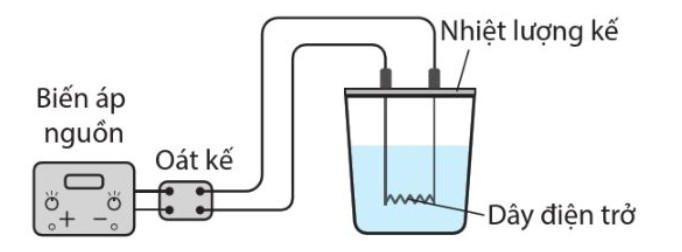
\includegraphics[scale=0.5]{figs/VN12-Y24-PH-SYL-004P-3}
}
\loigiai{
\begin{enumerate}[label=\alph*)]
	\item Đúng.
	\item Sai. Oát kế xác định công suất tiêu thụ điện của đoạn mạch.
	\item Đúng.
	\item Đúng.
\end{enumerate}
}
	\end{ex}

\begin{ex}
	Một chiếc thìa bằng đồng và một chiếc thìa bằng nhôm có cùng khối lượng và nhiệt độ ban đầu, được nhúng chìm vào cùng một cốc nước nóng (cao hơn nhiệt độ 2 thìa).
	\begin{enumerate}[label=\alph*)]
		\item 1 thìa toả nhiệt và 1 thìa thu nhiệt.
		\item Nhiệt độ cuối cùng của hai thìa bằng nhau.
		\item Khi có cân bằng nhiệt, nước bị giảm nhiệt độ.
		\item Nhiệt lượng của hai thìa trao đổi với nước là bằng nhau.
	\end{enumerate}
\loigiai{
\begin{enumerate}[label=\alph*)]
	\item Sai. Cả 2 thìa đều nhận nhiệt.
	\item Đúng.
	\item Đúng.
	\item Sai. Hai thìa có độ biến thiên nhiệt độ và khối lượng như nhau nhưng nhiệt dung riêng của chúng khác nhau nên nhiệt lượng trao đổi với nước của chúng khác nhau.
\end{enumerate}
}
	\end{ex}

\subsection{BÀI TẬP TỰ LUẬN}
\setcounter{ex}{0}
% ===================================================================
\begin{ex}
	\immini{
So sánh nhiệt dung riêng của thịt và của khoai tây, biết rằng khi cùng múc ra từ nồi canh hầm thì miếng thịt nguội nhanh hơn miếng khoai tây có cùng khối lượng.	

}{
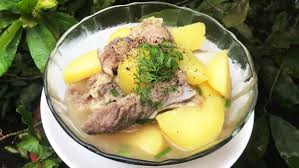
\includegraphics[scale=0.3]{figs/VN12-Y24-PH-SYL-004P-4}
}
\loigiai{
\begin{itemize}
	\item Nhiệt dung riêng là đại lượng thể hiện mức độ khó nóng, khó nguội của chất. Chất nào có nhiệt dung riêng lớn hơn thì khó nóng, khó nguội hơn.
	\item Khi cùng múc ra từ nồi canh hầm, miếng thịt nguội nhanh hơn miếng khoai tây cùng khối lượng. Điều này chứng tỏ thịt dễ nguội hơn khoai tây, nghĩa là nhiệt dung riêng của thịt nhỏ hơn nhiệt dung riêng của khoai tây.
\end{itemize}
}
	
	\end{ex}
% ===================================================================
\begin{ex}
Thùng nhôm khối lượng $\SI{1.2}{\kilogram}$ đựng $\SI{4}{\kilogram}$ nước ở $\SI{90}{\celsius}$. Cho biết nhiệt dung riêng của nhôm và nước lần lượt là $c_1=\SI{0.92}{\kilo\joule/\kilogram\cdot\kelvin}$, $c_2=\SI{4.186}{\kilo\joule/\left(\kilogram\cdot\kelvin\right)}$. Xác định nhiệt lượng thùng nước toả ra khi nhiệt độ giảm xuống còn $\SI{30}{\celsius}$.
	\loigiai{
	Nhiệt lượng do thùng nước toả ra:
	$$Q=\left(m_1c_1+m_2c_2\right)\Delta t=-\SI{1070880}{\joule}.$$
	Vậy nhiệt lượng do thùng nước toả ra là $\SI{1070880}{\joule}$.
	}
	
\end{ex}
% ===================================================================
\begin{ex}
	Để làm nguội nước nóng, người ta trộn $\SI{1.5}{\kilogram}$ nước ở $\SI{25}{\celsius}$ với $\SI{100}{\gram}$ nước ở $\SI{50}{\celsius}$. Xác định nhiệt độ cuối cùng của hỗn hợp khi cân bằng nhiệt.
	\loigiai{
	Khi có sự cân bằng nhiệt, tổng nhiệt lượng trao đổi trong hệ bằng 0:
	$$m_1c\left(t-t_1\right)+m_2c\left(t-t_2\right)=0$$
	$$\Leftrightarrow 1,5\left(t-\SI{25}{\celsius}\right)+0,1\left(t-\SI{50}{\celsius}\right)=0\Rightarrow t=\SI{26.5625}{\celsius}.$$
	}
	
\end{ex}
% ===================================================================
\begin{ex}
Muốn có nước ở nhiệt độ $t = \SI{50}{\celsius}$, người ta lấy $m_1 = \SI{3}{\kilogram}$ nước ở nhiệt độ $t_1 = \SI{100}{\celsius}$ trộn với nước ở nhiệt độ $t_2 =\SI{20}{\celsius}$. Hãy xác định khối lượng nước lạnh cần dùng.
	\loigiai{
		Khi cân bằng nhiệt, tổng nhiệt lượng trao đổi trong hệ bằng 0:
		$$m_1c\left(t_\text{cb}-t_1\right)+m_2c\left(t_\text{cb}-t_2\right)=0$$
		$$\Rightarrow m_2=\dfrac{m_1\left(t_1-t_\text{cb}\right)}{t_\text{cb}-t_2}=\SI{5}{\kilogram}.$$
	}
	
\end{ex}
% ===================================================================
\begin{ex}
Để xác định nhiệt dung riêng của một chất lỏng, người ta đổ chất lỏng đó vào $\SI{20}{\gram}$ nước ở nhiệt độ $\SI{100}{\celsius}$. Khi có cân bằng nhiệt, nhiệt độ của hỗn hợp đó là $\SI{37.5}{\celsius}$. Khối lượng hỗn hợp là $\SI{140}{\gram}$. Tính nhiệt dung riêng của chất lỏng đó, biết rằng nhiệt độ ban đầu của nó là $\SI{20}{\celsius}$ và hai chất lỏng không tác dụng hoá học với nhau. Cho nhiệt dung riêng của nước $c_2=\SI{4200}{\joule/\left(\kilogram\cdot\kelvin\right)}$.
	\loigiai{
	Gọi $m$ và $c$ lần lượt là khối lượng và nhiệt dung riêng của chất lỏng cần xác định nhiệt dung riêng.\\
	Khối lượng của chất lỏng đó:
	$$m=m_\text{hh}-m_\text{n}=\SI{120}{\gram}.$$
	Khi hệ đạt trạng thái cân bằng nhiệt thì tổng nhiệt lượng trao đổi của hệ bằng 0:
	$$mc\left(t_\text{cb}-t_0\right)+m_\text{n}c_\text{n}\left(t_\text{cb}-t_\text{0n}\right)=0$$
	$$\Rightarrow c=-\dfrac{m_\text{n}c_\text{n}\left(t_\text{cb}-t_\text{0n}\right)}{m\left(t_\text{cb}-t_0\right)}=\dfrac{\left(\SI{0.02}{\kilogram}\right)\cdot\left[\SI{4200}{\joule/\left(\kilogram\cdot\kelvin\right)}\right]\cdot\left(\SI{37.5}{\celsius}-\SI{100}{\celsius}\right)}{\left(\SI{0.12}{\kilogram}\right)\cdot\left(\SI{37.5}{\celsius}-\SI{20}{\celsius}\right)}=\SI{2500}{\joule/\left(\kilogram\cdot\kelvin\right)}.$$
	}
	
\end{ex}
% ===================================================================
\begin{ex}
	Để xác định nhiệt độ của một chiếc lò, người ta đốt nóng trong lò một cục sắt khối lượng $m_1=\SI{0.5}{\kilogram}$ rồi thả nhanh vào trong bình chứa $m_2=\SI{4}{\kilogram}$ nước có nhiệt độ ban đầu là $\SI{18}{\celsius}$. Nhiệt độ cuối cùng trong bình là $\SI{28}{\celsius}$. Hãy xác định nhiệt độ của lò. Bỏ qua trao đổi nhiệt với vỏ bình và quá trình nước hoá hơi khi tiếp xúc với cục sắt nóng. Cho nhiệt dung riêng của sắt là $c_1=\SI{460}{\joule/\left(\kilogram\cdot\kelvin\right)}$, nhiệt dung riêng của nước là $c_2=\SI{4200}{\joule/\left(\kilogram\cdot\kelvin\right)}$.
	\loigiai{
	Khi cân bằng nhiệt, tổng nhiệt lượng trao đổi trong hệ bằng 0:
	$$m_1c_1\left(t_\text{cb}-t_1\right)+m_2c_2\left(t_\text{cb}-t_2\right)=0\Rightarrow t_1\approx\SI{758.4}{\celsius}.$$
	}
	
\end{ex}
% ===================================================================
\begin{ex}
Trộn lẫn rượu vào nước, người ta thu được một hỗn hợp nặng $\SI{120.8}{\gram}$ ở nhiệt độ $\SI{30}{\celsius}$. Tính khối lượng nước và rượu đã pha, biết rằng ban đầu rượu ở nhiệt độ $\SI{10}{\celsius}$ và nước ở nhiệt độ $\SI{90}{\celsius}$. Cho nhiệt dung riêng của rượu và nước lần lượt là $\SI{2500}{\joule/\left(\kilogram\cdot\kelvin\right)}$, $\SI{4200}{\joule/\left(\kilogram\cdot\kelvin\right)}$.
	\loigiai{
		Gọi:
		\begin{itemize}
			\item $m_1, c_1, t_1$ lần lượt là khối lượng, nhiệt dung riêng và nhiệt độ ban đầu của rượu;
			\item $m_2, c_2, t_2$ lần lượt là khối lượng, nhiệt dung riêng và nhiệt độ ban đầu của nước.
		\end{itemize}
		Ta có:
		\begin{equation}
			\label{eq:4P-1}
			m_1+m_2=\SI{120.8}{\gram}=\SI{0.1208}{\kilogram}
		\end{equation}
		Khi hệ cân bằng nhiệt, tổng nhiệt lượng trao đổi trong hệ bằng 0:
		$$m_1c_1\left(t_\text{cb}-t_1\right)+m_2c_2\left(t_\text{cb}-t_2\right)=0$$
		\begin{equation}
			\label{eq:4P-2}
			50000m_1-252000m_2=0
		\end{equation}
		Từ (\ref{eq:4P-1}) và (\ref{eq:4P-2}) suy ra:
		\begin{equation*}
			\begin{cases}
				m_1=\SI{100.8}{\gram}\\
				m_2=\SI{20}{\gram}
			\end{cases}
			.
		\end{equation*}
	}
	
\end{ex}
% ===================================================================
\begin{ex}
	Bỏ một vật rắn khối lượng $\SI{100}{\gram}$ ở $\SI{100}{\celsius}$ vào $\SI{500}{\gram}$ nước ở $\SI{15}{\celsius}$ thì nhiệt độ sau cùng của vật là $\SI{16}{\celsius}$. Thay nước bằng $\SI{800}{\gram}$ chất lỏng khác ở $\SI{10}{\celsius}$ thì nhiệt độ sau cùng là $\SI{13}{\celsius}$. Tìm nhiệt dung riêng của vật rắn và chất lỏng. Cho nhiệt dung riêng của nước là $c = \SI{4200}{\joule/\left(\kilogram\cdot\kelvin\right)}$.
	\loigiai{
		\textbf{Khi bỏ vật rắn vào nước:}\\
		Khi cân bằng nhiệt, tổng nhiệt lượng trao đổi của vật rắn và nước bằng 0:
		$$m_vc_v\left(t_\text{cb}-t_v\right)+m_nc_n\left(t_\text{cb}-t_n\right)=0\Rightarrow c_v=\dfrac{m_nc_n\left(t_\text{cb}-t_n\right)}{m_v\left(t_v-t_\text{cb}\right)}=\SI{250}{\joule/\left(\kilogram\cdot\kelvin\right)}.$$
		\textbf{Khi bỏ vật rắn vào trong chất lỏng khác}\\
		Khi cân bằng nhiệt, tổng nhiệt lượng trao đổi của vật rắn và chất lỏng bằng 0:
		$$m_vc_v\left(t'_\text{cb}-t_v\right)+m_lc_l\left(t'_\text{cb}-t_l\right)\Rightarrow c_l=\dfrac{m_vc_v\left(t_v-t_\text{cb}\right)}{m_l\left(t'_\text{cb}-t_l\right)}=\SI{906.25}{\joule/\left(\kilogram\cdot\kelvin\right)}.$$
	}
	
\end{ex}
% ===================================================================
\begin{ex}
Người ta đổ $m_1 =\SI{200}{\gram}$ nước sôi có nhiệt độ $t_1 =\SI{100}{\celsius}$ vào một chiếc cốc có khối lượng $m_2 = \SI{120}{\gram}$ đang ở nhiệt độ $t_2 =\SI{20}{\celsius}$. sau khoảng thời gian $T = \SI{5}{\text{phút}}$, nhiệt độ của cốc nước bằng $t=\SI{40}{\celsius}$. Xem rằng sự mất nhiệt xảy ra một cách điều đặn, hãy xác định nhiệt lượng tỏa ra môi trường xung quanh trong mỗi giây. Cho nhiệt dung riêng nước và thuỷ tinh lần lượt là $c_1=\SI{4200}{\joule/\left(\kilogram\cdot\kelvin\right)}$, $c_2=\SI{840}{\joule/\left(\kilogram\cdot\kelvin\right)}$.
	\loigiai{Nhiệt lượng nước sôi toả ra để giảm nhiệt độ từ $\SI{100}{\celsius}$ còn $\SI{40}{\celsius}$:
		$$Q_\text{toả}=m_1c_1\left(t_1-t\right)=\SI{50400}{\joule}.$$
		Nhiệt lượng cốc thuỷ tinh thu vào để tăng nhiệt độ từ $\SI{20}{\celsius}$ lên $\SI{40}{\celsius}$:
		$$Q_\text{thu}=m_2c_2\left(t-t_2\right)=\SI{2016}{\joule}.$$
		Nhiệt lượng toả ra môi trường trong mỗi giây:
		$$w=\dfrac{Q_\text{toả}-Q_\text{thu}}{T}=\SI{161.28}{\joule/\second}.$$
	}
	
\end{ex}
% ===================================================================
\begin{ex}
	Trộn ba chất lỏng không tác dụng hoá học với nhau có khối lượng lần lượt là $m_1=\SI{2}{\kilogram}$, $m_2=\SI{3}{\kilogram}$, $m_3=\SI{4}{\kilogram}$. Biết nhiệt dung riêng và nhiệt độ ban đầu của mỗi chất lỏng lần lượt là $c_1=\SI{2000}{\joule/\left(\kilogram\cdot\kelvin\right)}$, $t_1=\SI{57}{\celsius}$, $c_2=\SI{4000}{\joule/\left(\kilogram\cdot\kelvin\right)}$, $t_2=\SI{63}{\celsius}$, $c_3=\SI{3000}{\joule/\left(\kilogram\cdot\kelvin\right)}$, $t_3=\SI{92}{\celsius}$. Nhiệt độ của hỗn hợp khi cân bằng nhiệt là bao nhiêu?
	\loigiai{Khi cân bằng nhiệt, tổng nhiệt lượng trao đổi trong hệ bằng 0:
		$$m_1c_1\left(t_\text{cb}-t_1\right)+m_2c_2\left(t_\text{cb}-t_2\right)+m_3c_3\left(t_\text{cb}-t_3\right)=0$$
		$$\Rightarrow t_\text{cb}=\dfrac{m_1c_1t_1+m_2c_2t_2+m_3c_3t_3}{m_1c_1+m_2c_2+m_3c_3}\approx\SI{74.6}{\celsius}.$$
	}
	
\end{ex}
% ===================================================================
\begin{ex}
	Một nhiệt lượng kế bằng nhôm có khối lượng $m_1 = \SI{100}{\gram}$ chứa $m_2 =\SI{400}{\gram}$ nước ở nhiệt độ $t_1 =\SI{10}{\celsius}$. Người ta thả vào nhiệt lượng kế một thỏi hợp kim nhôm và thiếc có khối lượng $m = \SI{200}{\gram}$ được nung nóng đến nhiệt độ $t_2 =\SI{120}{\celsius}$. Nhiệt độ cân bằng của hệ thống là $\SI{14}{\celsius}$. Tính khối lượng nhôm và thiếc có trong hợp kim. Cho nhiệt dung riêng của nhôm, nước, thiếc lần lượt là: $c_1 =\SI{900}{\joule/\left(\kilogram\cdot\kelvin\right)}$, $c_2=\SI{4200}{\joule/\left(\kilogram\cdot\kelvin\right)}$, $c_3 =\SI{230}{\joule/\left(\kilogram\cdot\kelvin\right)}$.
	\loigiai{Gọi $m_\text{nh}$, $m_\text{th}$ lần lượt là khối lượng của nhôm và thiếc trong hợp kim.\\
		Ta có:
		\begin{equation}
			\label{eq:4P-3}
			m_\text{nh}+m_\text{th}=\SI{0.2}{\kilogram}
		\end{equation}
		Khi hệ cân bằng nhiệt, tổng nhiệt lượng trao đổi trong hệ bằng 0:
		$$m_1c_1\left(t_\text{cb}-t_1\right)+m_2c_2\left(t_\text{cb}-t_1\right)+m_\text{nh}c_1\left(t_\text{cb}-t_2\right)+m_\text{th}c_3\left(t_\text{cb}-t_2\right)=0$$
		\begin{equation}
			\label{eq:4P-4}
			95400m_\text{nh}+24380m_\text{th}=7080
		\end{equation}
		Từ (\ref{eq:4P-3}) và (\ref{eq:4P-4}), suy ra:
		\begin{equation*}
			\begin{cases}
				m_\text{nh}\approx\SI{0.031}{\kilogram}\\
				m_\text{th}\approx\SI{0.169}{\kilogram}
			\end{cases}
		\end{equation*}
	}
	
\end{ex}
% ===================================================================
\begin{ex}
	Một khối sắt có khối lượng $m$ ở nhiệt độ $\SI{150}{\celsius}$ khi thả vào một bình nước thì làm nhiệt độ nước tăng từ $\SI{20}{\celsius}$ lên $\SI{60}{\celsius}$. Thả tiếp vào nước khối sắt thứ hai có khối lượng $\dfrac{m}{2}$ ở $\SI{100}{\celsius}$ thì nhiệt độ sau cùng của nước là bao nhiêu? Coi như chỉ có sự trao đổi nhiệt giữa khối sắt với nước và bỏ qua quá trình nước hoá thành hơi khi tiếp xúc với sắt nóng.
	\loigiai{	Gọi:
		\begin{itemize}
			\item $m_2$ là khối lượng nước trong bình;
			\item $c_1$, $c_2$ lần lượt là nhiệt dung riêng của sắt và nước;
			\item $t_1$, $t_2$ lần lượt là nhiệt độ ban đầu của thỏi sắt khối lượng $m$ và nước.
		\end{itemize}
		\textbf{Bỏ khối sắt khối lượng $m$ vào nước}\\
		Khi có cân bằng nhiệt, nhiệt lượng trao đổi trong hệ bằng 0:
		$$mc_1\left(t_\text{cb}-t_1\right)+m_2c_2\left(t_\text{cb}-t_2\right)=0\Rightarrow \dfrac{mc_1}{m_2c_2}=\dfrac{t_\text{cb}-t_2}{t_1-t_\text{cb}}=\dfrac{4}{9}.$$
		\textbf{Bỏ thêm khối sắt khối lượng $m/2$ vào nước}\\
		Khi có cân bằng nhiệt, nhiệt lượng trao đổi trong hệ bằng 0:
		$$\left(mc_1+m_2c_2\right)\left(t'_\text{cb}-t_\text{cb}\right)+\dfrac{m}{2}c_1\left(t'_\text{cb}-t'_1\right)=0$$
		$$\Rightarrow \Rightarrow t'_\text{cb}=\dfrac{mc_1\left(t_\text{cb}+\dfrac{t'_1}{2}\right)+m_2c_2t_\text{cb}}{1,5mc_1+m_2c_2}=\dfrac{\dfrac{4}{9}\cdot\left(\SI{60}{\celsius}+\SI{50}{\celsius}\right)+\SI{60}{\celsius}}{1,5\cdot\dfrac{4}{9}+1}\approx\SI{65.33}{\celsius}.$$
	}
	
\end{ex}
% ===================================================================
\begin{ex}
Có hai bình cách nhiệt. Bình 1 chứa $m_1 =\SI{2}{\kilogram}$ nước ở $t_1=\SI{20}{\celsius}$, bình 2 chứa $m_2 =\SI{4}{\kilogram}$ nước ở $t_2 =\SI{60}{\celsius}$. Người ta rót một lượng nước $m$ từ bình 1 sang bình 2, sau khi cân bằng nhiệt, người ta lại rót một lượng nước từ bình 2 sang bình 1. Nhiệt độ cân bằng ở bình 1 lúc này là $\SI{21.95}{\celsius}$.
\begin{enumerate}[label=\alph*)]
	\item Tính lượng nước $m$ rong mỗi lần rót và nhiệt độ cân bằng ở bình 2.
	\item Nếu tiếp tục thực hiện lần hai, tìm nhiệt độ cân bằng ở mỗi bình.
\end{enumerate}
	\loigiai{\begin{enumerate}[label=\alph*)]
			\item \begin{itemize}
				\item \textbf{Rót nước từ bình 1 sang bình 2}\\
				Khi cân bằng nhiệt, tổng nhiệt lượng trao đổi của $m$ và lượng nước ở bình 2 bằng 0:
				$$mc\left(t'_2-t_1\right)+m_2c\left(t'_2-t_2\right)=0$$
				\begin{equation}
					\label{eq:4P-5}
					m\left(t'_2-t_1\right)=m_2\left(t_2-t'_2\right)
				\end{equation}
				\item \textbf{Rót nước từ bình 2 sang bình 1}\\
				Khi cân bằng nhiệt, tổng nhiệt lượng trao đổi của $m$ và lượng nước ở bình 1 bằng 0:
				$$mc\left(t'_1-t\right)+\left(m_1-m\right)c\left(t'_1-t_1\right)=0$$
				\begin{equation}
					\label{eq:4P-6}
					m\left(t-t_1\right)=m_1\left(t'_1-t_1\right)
				\end{equation}
				Từ (\ref{eq:4P-5}) và (\ref{eq:4P-6}), suy ra:
				\begin{equation*}
					\begin{cases}
						t=\dfrac{m_2t_2-m_1\left(t'_1-t_1\right)}{m_2}\approx\SI{59}{\celsius}\\
						m=\dfrac{m_1m_2\left(t'_1-t_1\right)}{m_2\left(t_2-t_1\right)-m_1\left(t'_1-t_1\right)}\approx\SI{0.1}{\kilogram}
					\end{cases}
					.
				\end{equation*}
			\end{itemize}
			\item Thực hiện lần hai, nhiệt độ cân bằng của mỗi bình là
			$$t''_2=\dfrac{mt'_1+m_2t'_2}{m+m_2}=\SI{58.12}{\celsius};\quad t''_1=\dfrac{mt''_2+\left(m_1-m\right)t_1}{m_1}=\SI{23.76}{\celsius}.$$
		\end{enumerate}
	}
	
\end{ex}